%; whizzy chapter
% -initex iniptex -latex platex -format platex -bibtex jbibtex -fmt fmt
% $B0J>e(B whizzytex $B$r;HMQ$9$k>l9g$N@_Dj!#(B

%     Kansai Debian Meeting resources
%     Copyright (C) 2007 Takaya Yamashita
%     Thank you for Tokyo Debian Meeting resources

%     This program is free software; you can redistribute it and/or modify
%     it under the terms of the GNU General Public License as published by
%     the Free Software Foundation; either version 2 of the License, or
%     (at your option) any later version.

%     This program is distributed in the hope that it will be useful,
%     but WITHOUT ANY WARRANTY; without even the implied warranty of
%     MERCHANTABILITY or FITNESS FOR A PARTICULAR PURPOSE.  See the
%     GNU General Public License for more details.

%     You should have received a copy of the GNU General Public License
%     along with this program; if not, write to the Free Software
%     Foundation, Inc., 51 Franklin St, Fifth Floor, Boston, MA  02110-1301 USA

%  preview (shell-command (concat "evince " (replace-regexp-in-string "tex$" "pdf"(buffer-file-name)) "&"))
% $B2hA|%U%!%$%k$r=hM}$9$k$?$a$K$O(Bebb$B$rMxMQ$7$F(Bboundingbox$B$r:n@.!#(B
%(shell-command "cd image200708; ebb *.png")

%%$B$3$3$+$i%X%C%@3+;O!#(B

\documentclass[mingoth,a4paper]{jsarticle}
\usepackage{kansaimonthlyreport}
\usepackage[dvips]{xy}


% $BF|IU$rDj5A$9$k!"Kh7nJQ$o$j$^$9!#(B
\newcommand{\debmtgyear}{2012}
\newcommand{\debmtgdate}{25}
\newcommand{\debmtgmonth}{3}
\newcommand{\debmtgnumber}{57}

\begin{document}

\begin{titlepage}

% $BKh7nJQ99$9$kItJ,!"K\J8$NKvHx$b=$@5$9$k$3$H$r$o$9$l$:$K(B

 $BBh(B\debmtgnumber{}$B2s(B $B4X@>(B Debian $BJY6/2q;qNA(B

\vspace{2cm}

\begin{center}
\includegraphics{image200802/kansaidebianlogo.png}
\end{center}

\begin{flushright}
\hfill{}$B4X@>(B Debian $BJY6/2qC4Ev<T(B $B:4!9LZ!&ARI_!&$N$,$?!&$+$o$@(B \\
\hfill{}\debmtgyear{}$BG/(B\debmtgmonth{}$B7n(B\debmtgdate{}$BF|(B
\end{flushright}

\thispagestyle{empty}
\end{titlepage}

\dancersection{Introduction}{Debian JP}

 $B4X@>(BDebian$BJY6/2q$O(BDebian GNU/Linux$B$N$5$^$6$^$J%H%T%C%/(B
 ($B?7$7$$%Q%C%1!<%8!"(BDebian$BFCM-$N5!G=$N;EAH!"(BDebian$B3&7($G5/$3$C$?=PMh;v!"(B
 $B$J$I$J$I!K$K$D$$$FOC$79g$&2q$G$9!#(B

 $BL\E*$H$7$F<!$N;0$D$r9M$($F$$$^$9!#(B
 \begin{itemize}
  \item ML$B$d7G<(HD$G$O$J$/!"D>@\4i$r9g$o$;$k;v$G$N>pJs8r49$NB%?J(B
  \item $BDj4|E*$K=8$^$l$k>l=j(B
  \item $B;qNA$N:n@.(B
 \end{itemize}

 $B$=$l$G$O!"3Z$7$$0l;~$r$*3Z$7$_2<$5$$!#(B

\newpage

\begin{minipage}[b]{0.2\hsize}
 {\rotatebox{90}{\fontsize{80}{80}
{\gt $B4X@>(B Debian $BJY6/2q(B}}}
\end{minipage}
\begin{minipage}[b]{0.8\hsize}
\hrule
\vspace{2mm}
\hrule
\setcounter{tocdepth}{1}
\tableofcontents
\vspace{2mm}
\hrule
\end{minipage}

\dancersection{$B:G6a$N(BDebian$B4X78$N%$%Y%s%HJs9p(B}{Debian JP}

\clearpage

\dancersection{$B;vA02]Bj(B}{Debian JP}

$B:#2s$O0J2<$N2]Bj$r=PBj$7$^$7$?(B.
\begin{screen}
  \begin{enumerate}
  \item Debian Policy $B$NBh(B5$B>O$rFI$s$G$-$F2<$5$$!#(B
  \item $B2?$+0l$D%Q%C%1!<%8$r<hF@$7$F(B debian/control $B%U%!%$%k$rFI$s$G$-$F$/$@$5$$!#(B
    \begin{itemize}
    \item $B$=$N%Q%C%1!<%8$N(B control $B%U%!%$%k$NFbMF$K$D$$$F4JC1$K!"$o$+$i$J$$2U=j$OD4$Y$F!"EvF|>R2p$7$F2<$5$$!#(B
    \end{itemize}
  \item $BJY6/2q3+:E$r$I$N$h$&$JG^BN!"J}K!$G9pCN$r=P$7$F$b$i$$$?$$$G$9$+!#(B
  \end{enumerate}
\end{screen}

$B;22C<T$N3'$5$s$N2rEz$O0J2<$NDL$j$G$9(B.

\clearpage

\dancersection{$B?7G/EY%9%1%8%e!<%k$K4X$7$F(B}{$B:4!9LZMNJ?(B}

\clearpage

\dancersection{Konoha $B$N(B Debian$B%Q%C%1!<%82=$K$D$$$F(B}{$B<r0f(B $BCi5*(B}
\subsection{$B$O$8$a$K(B}
Konoha $B$r(B Debian $B%Q%C%1!<%8$K$7$F(B sid $B$K%3%_%C%H$7$?$$$H9M$($F$$$^$9!#(B
$B:#2s$O!"0J2<$K$D$$$F@bL@$7$^$9!#(B
\begin{itemize}
\item Konoha $B$N35MW(B
\item $B%Q%C%1!<%82=$NFbMF3NG'(B
\item $B%9%]%s%5!<$K$J$C$F$/$@$5$kJ}$NAjCL(B
\end{itemize}

\subsection{Konoha $B$N35MW(B}

\subsubsection{Konoha $B$H$O(B}
Konoha $B$O!"@EE*7?IU$1$K$h$k%*%V%8%'%/%H;X8~%9%/%j%W%H8@8l$G$9!#(B
$B2#IM9qN)Bg3X$H(B JST/DEOS $B%W%m%8%'%/%H$rCf?4$K%*!<%W%s%=!<%9$G3+H/$5$l$F(B
$B$$$^$9!#(B
\footnote{$B;d$O(B Konoha $B%W%m%8%'%/%HFbIt$N?M4V$G$O$J$$$N$G!"0J2<$N5-=R$O@5$7$/$J$$>l9g$,$"$k$+$b$7$l$^$;$s!#(B}

\begin{quote}
$B3+H/%5%$%H(B: \url{http://konoha.sourceforge.jp}
\end{quote}

Konoha $B$O!"@EE*8@8l$N8@8l5;=Q$r4pHW$H$7$F!"$=$N>e$KF0E*$J?6$kIq$$$r%b%G(B
$B%k2=$7$F$$$^$9!#(B

$B0J2<$K5-=R$9$k$h$&$K!"%9%/%j%W%H$H$7$F<B9T$9$k$3$H$d!"%3%s%Q%$%i8@8l$N(B
$B$h$&$K<B9TA0$K7?8!::$r9T$&$3$H$,$G$-$^$9!#(B

\begin{itemize}
\item $B%9%/%j%W%H$H$7$F<B9T(B

$B4X?t$r=q$-;O$a$?;~E@$G$O7?$d%/%i%93,AX$OL@3N$K7h$^$C$F$*$i$:!"8e$+$i(B
$BIQHK$K=q$-49$($F!"%"%$%G%"$,8G$^$C$F$+$i7?$d%/%i%93,AX$r7h$a$?$$>l9g(B
$B$,$"$j$^$9!#(B

Konoha $B$O@EE*8@8l$G$"$j$J$,$i2DG=$J8B$jF0E*8@8l$N?6$kIq$$$r%(%_%e%l!<(B
$B%7%g%s$7!"4X?t$,:G=i$K8F$S=P$5$l$kD>A0$K%Q%i%a!<%?$+$i7?$r?dO@$7!"CY(B
$B1d%3%s%Q%$%k$7$^$9!#(B

$B$7$?$,$C$F!"@EE*8@8l$G$"$j$J$,$i%9%/%j%W%H8@8l$N$h$&$K7?Dj5A$J$I$r>J(B
$BN,$7$F<B9T$9$k$3$H$,$G$-!"=@Fp$K3+H/$r?J$a$k$3$H$,$G$-$^$9!#(B

\item $B<B9TA0$N7?8!::(B

$B=>Mh$N%9%/%j%W%H8@8l$N$h$&$K!"F0E*$J7?8!::$r%Y!<%9$K$7$F$$$k$H!"7?%((B
$B%i!<$,4^$^$l$k%9%/%j%W%H$G$b<B9T$7$J$$$H%(%i!<$,H/8+$G$-$^$;$s!#(B

$B$=$N$?$a!"A4$F$N<B9T%Q%9$r$R$H$D$R$H$D%F%9%H<B9T$7$J$,$i!"7?%(%i!<$r(B
$BC5$7!"=$@5$9$kI,MW$,$"$j$^$9!#(B

Konoha $B$O@EE*$J7?IU$18@8l$G$"$k$?$a!"%W%m%0%i%`$rF0:n$5$;$k$3$H$J$/!"(B
$B7?8!::$r9T$&$3$H$,$G$-!"=iJbE*$J%(%i!<$r8!>Z$9$k$3$H$,$G$-$^$9!#(B

$B$=$N$?$a!"%1%"%l%9%_%9$N$?$a$K!"%U%!%$%kA`:n$d%G!<%?%Y!<%9$,CfESH>C<(B
$B$J>uBV$K$J$j!"%W%m%0%i%`$,Dd;_$9$kJ@32$b$"$j$^$;$s!#(B

\end{itemize}

Konoha $B$r>u67$K9g$o$;$F;HMQJ}K!$r;H$$J,$1$k$3$H$G!"$R$H$D$N8@8l$G@EE*8@(B
$B8l$H%9%/%j%W%H8@8l$NFCD'$r@8$+$7$?3+H/$r9T$&$3$H$,$G$-$^$9!#(B

$B$3$l$O!"<!$N$h$&$J>l9g$KM-8z$K3hMQ$G$-$k$H9M$($^$9!#(B

$B%"%W%j%1!<%7%g%s3+H/$K$*$$$F!"0J2<$N$h$&$J<j=g$G9T$o$l$k>l9g$,$"$k$H;W(B
$B$$$^$9!#(B

\begin{itemize}
\item STEP1: $B%9%/%j%W%H8@8l$rMQ$$$?%W%m%H%?%$%W$N:n@.(B

$B7?@k8@$d%/%i%9@_7W$O8e2s$7$K$7$F!"=SIR$K%"%$%G%"$r%3!<%I2=$9$k(B

\item STEP2: $B@EE*8@8l$G=q$-D>$7(B

$BIJ<AJ]>Z!"%a%s%F%J%s%9@-$N8~>e(B
\end{itemize}
  
$B$7$+$7!"0lC6@EE*8@8l$G=q$-D>$7$F$7$^$&$H!"%9%/%j%W%H8@8l$N$h$&$K=@Fp$K(B
$B=q$-D>$7$,$G$-$J$/$J$j$^$9!#(B

Konoha $B$r;HMQ$9$l$P!">e5-$N(B STEP1 $B$H(B STEP2 $B$r7+$jBX$($7$F3+H/$r?J$a$k$3(B
$B$H$,$G$-$^$9!#(B

Konoha $B$O%9%/%j%W%H8@8l$,Ds6!$9$k=@Fp$5$H@EE*8@8l$,;}$DIJ<AJ]>Z$rN>N)$5(B
$B$;$k$3$H$rL\;X$7$F$$$^$9!#(B

\subsubsection{Konoha $B$N;H$$J}(B}
\begin{enumerate}
\item $BBPOC%b!<%I(B
Konoha $B$O%?!<%_%J%k$+$i(B Konoha $B%3%^%s%I$r<B9T$9$k$H!"BPOC%7%'%k$H$7$F5/(B
$BF0$7$^$9!#(B

\begin{commandline}
$ konoha
konoha 1.0(beta) svn (rev:933, Mar 23 2012 05:37:24)
options: iconv bmgc thcode sqlite3 syslog thread used\_memory:2191 kb
SECURITY ALERT: ** FOR EVALUATION/DEVELOPMENT USE ONLY **

>>>
nd{commandline}

"$>>>$" $B$O!"BPOC%7%'%k$N%W%m%s%W%H$G$9!#$3$N>uBV$G<B9T$7$?$$%W%m%0%i%`$r(B
$BF~NO$9$k$H!"<!$N9T$K<B9T7k2L$,I=<($5$l$^$9!#(B

\begin{commandline}
>>> print "hello, Konoha!"
((eval):1) hello, Konoha!
\end{commandline}

$BBPOC%7%'%k$r=*N;$7$?$$>l9g$O!"(B"bye" $B$b$7$/$O(B (Conrol-D) $B$rF~NO$7$^$9!#(B

\begin{commandline}
>>> bye
\end{commandline}

\item $B%9%/%j%W%H%b!<%I(B
Konoha $B$O%W%m%0%i%`$r%U%!%$%k$KJ]B8$9$l$P!"%9%/%j%W%H$H$7$F<B9T$G$-$^$9!#(B

\begin{commandline}
$ cat <<EOF > fact.k
int factorial(int n) {
  if(n == 1) return 1;
  return n * factorial(n - 1);
}
print factorial(10);
EOF

$ konoha fact.k
(fact.k:5) 3628800
\end{commandline}

$B$^$?!"(B-i$B%*%W%7%g%s$rIU$1$F(B Konoha $B$r5/F0$9$l$P!"%9%/%j%W%H%U%!%$%k$rFI(B
$B$_9~$s$@8e!"BPOC%7%'%k$+$iDj5A$5$l$?4X?t$rMxMQ$G$-$^$9!#(B

\clearpage

\item $B%9%/%j%W%H$N<B9TA0$N7?8!::(B
$B7?8!::$N$_<B9T$9$k>l9g$O!"(B-c$B%*%W%7%g%s$rIU$1$F(B Konoha $B$r5/F0$7$^$9!#(B

\begin{commandline}
$ cat <<EOF > type-error.k
s = 'ever';
i = 4;
str = i + s;    // $B7??dO@(B
print str;      // "4ever" $B$HI>2A$5$l$k(B

int x = i + s;  // $B7?%(%i!<$H$J$k(B
print x;
EOF

$ konoha -c type-error.k
- (type-error.k:1) (info) suppose s has String type
- (type-error.k:2) (info) suppose i has int type
- (type-error.k:3) (info) suppose str has String type
- (type-error.k:6) (error) x has type int, not String
- (type-error.k:7) (error) undefined variable: x
\end{commandline}

\end{enumerate}

\subsubsection{Konoha $B$NFCD'(B}
Konoha $B$N<g$JFCD'$r0J2<$K5-=R$7$^$9!#(B
\begin{enumerate}
\item $B@EE*7?IU$1(B

$B7?$NBEEv@-$,J]>Z$5$l$F$$$^$9!#(B
$B%9%/%j%W%H<B9TA0$K7?8!::$N$_9T$&$3$H$,$G$-$^$9!#(B

\item $B7?@k8@$N>JN,(B($B7??dO@$dCY1d%3%s%Q%$%k(B)

$B0J2<$N>l9g!":G=i$K8F$S=P$5$l$k$N$,(B dsucc(1.0) $B$J$N$G0z?t$HLa$jCM$O(B
float$B7?$K7hDj$5$l$^$9!#(B

\begin{commandline}
function dsucc(n) {
  return n + 1;
}

dsucc(dsucc(1.0) + 1);
\end{commandline}

Konoha $B$O0lC6!"7?$,7hDj$7$?$i7?$N0l4S@-$rJ]>Z$7$^$9!#(B
$B$D$^$j!"<!$K(B dsucc("Konoha") $B$N$h$&$J0[$J$k7?$N8F$S=P$7$O7?%(%i!<$H$J(B
$B$j$^$9!#(B
$B$3$l$K$h$j@EE*8@8l$HF1$8$h$&$K7?%(%i!<$N4IM}$,$G$-$^$9!#(B
\\
\item $B@)8f$5$l$?F0E*7?IU$1(B(dynamic type)

Konoha $B$O%9%/%j%W%H8@8l$N$h$&$J%@%C%/%?%$%T%s%0$r%5%]!<%H$7$F$$$^$9!#(B

$B0J2<$N$h$&$K!"(Bdynamic$B7?$rMQ$$$k$H!"(B+$B1i;;;R$r%5%]!<%H$7$?G$0U$NCM$r=h(B
$BM}$G$-$^$9!#(B

\begin{commandline}
function dsucc(dynamic n) {
  return n + 1;
}
\end{commandline}

+$B1i;;;R$r%5%]!<%H$7$F$$$J$$CM$,M?$($i$l$k$H!"<B9T;~$N%(%i!<$H$J$j$^$9!#(B
dynamic$B7?$r@k8@$9$k(B/$B$7$J$$$G%(%i!<$NH/@8$r@)8f$G$-$^$9!#(B
\\
\item $B7ZNL$J%*%V%8%'%/%H(B

Konoha $B$O%3%s%9%H%i%/%?$,$J$/$F$b%*%V%8%'%/%H$N@8@.$,$G$-$^$9!#(B
$B$^$?!"(Bsetter/getter$B$O<+F0E*$K@8@.$5$l$^$9!#(B
\\
\item $BHFMQ@-$N9b$$=8Ls%G!<%?9=B$(B(Array, Map, Tuple)

\begin{commandline}
  Array($B%j%9%H(B)   ["naruto", 17]
  Map($B<-=q(B)       {name:"naruto", age:17}
  Tuple          ("naruto", 17)
\end{commandline}

\item $B<B9T;~$N%3%s%Q%$%k$HI>2A(B(eval)

$B%9%/%j%W%H8@8l$H$7$F<B9T$G$-$^$9!#(B

\clearpage

\item $B<B9T;~$N%/%i%9$N2~JQ(B

$B%a%=%C%I$O!"4{$K%*%V%8%'%/%H$,@8@.$7$F$"$C$F$b!"<B9T;~$K%/%i%9$KDI2C(B
$B$9$k$3$H$,$G$-$^$9!#(B
\\
\item $BIT40A4%3!<%I$NItJ,E*$J<B9T(B

$B=>Mh$N%3%s%Q%$%i5;=Q$G$O!"<B9TA0$K7?8!::$r9T$&$?$a!"<!$N$h$&$J7?%(%i!<(B
$B$,$"$k>l9g!"%3!<%I@8@.$,40N;$;$:!"%W%m%0%i%`$b<B9T$G$-$^$;$s$G$7$?!#(B

\begin{commandline}
int serial(int n) {
  if(n == 0) {
    InputStream in = new ("serial.txt");
    n = in.readLine(); // $B7?%(%i!<$,$3$3$K$"$k(B
    in.close();
  }
  return n + 1;
}
\end{commandline}

Konoha $B$G$O!"%3%s%Q%$%k;~$K%(%i!<$,H/@8$7$F$b!"$=$NItJ,$r<B9T;~Nc30$K(B
$B=q$-49$($k$3$H$,$G$-$^$9!#(B
$BNc$($P!">e5-$N7?%(%i!<$O<!$N%3!<%I$KJQ49$5$l$^$9!#(B

\begin{commandline}
int serial(int n) {
  if(n == 0) { // $BNc30$K$J$k(B
    throw new Script!!("");
  }
  return n + 1;
}
\end{commandline}

$B%(%i!<2U=j$r<B9T$7$J$1$l$P!"$=$N$^$^<B9T$,2DG=$G$"$j!"$b$7$b(B
serial(0) $B$r<B9T$7$F$b!"<B9T;~Nc30$H$7$F=hM}$G$-$^$9!#(B

\begin{commandline}
>>> serial(1)
2

>>> serian(0)
Script!!:
\end{commandline}

\item $BE}0lE*$J%G!<%?JQ49A`:n(B
Konoha $B$K$O!"%-%c%9%H1i;;;R$r3HD%$7$?%H%i%s%9%-%c%C%H$H8F$P$l$k%G!<%?(B
$BJQ49$rE}0lA`:n$G9T$&1i;;;R$,$"$j$^$9!#(B

\begin{commandline}
>>> (to String)1
"1"

>>> (to int)1
1

>>> (to int)"naruto"
null
\end{commandline}

$BJ8;zNs$X$NJQ49$O!"%U%)!<%^%C%?$N5!G=$rMQ$$$k$H!"MM!9$J=q<0$NJ8;zNs$K(B
$BJQ49$G$-$^$9!#(B

\begin{commandline}
>>> "%x"(-1)
"ffffffffffffffff"

>>> "%bits"(-1)
"11111111 11111111 11111111 11111111 11111111 11111111 11111111 11111111"
\end{commandline}

$BB>$K$b?'!9$JJQ495!G=$,$"$j$^$9!#(B
\\
\item $B%j%s%/1i;;;R$H30It%j%=!<%9$N07$$(B

Konoha $B$K$O30It%j%=!<%9$N<1JL;R$rD>@\07$&(B URN $B$,$"$j$^$9!#(B

\begin{quote}
    http://konohascript.org/\\
    file:/etc/passwd\\
    isbn:978-4-06-372988-7
\end{quote}

$B$^$?!"(BKonoha $B$O(B URN $B$+$iD>@\%j%=!<%9$rF@$k$3$H$,$G$-$^$9!#(B
"file:" $B$d(B "http:" $B$J$I$N(B URN $B%9%-!<%`$O!"%9%H%j!<%`$K7?6/@)$5$l$^$9!#(B
URN $B$rMQ$$$l$P!"<!$N$h$&$K=q$1$^$9!#(B

\begin{commandline}
foreach(String line from file:/etc/hosts) {
  print line;
}
\end{commandline}

\item $BHs6&M-%G!<%?%b%G%k(B($B%"%/%?!<(B)$B$K$h$kJB9T=hM}(B

  ???\footnote{$B?=$7Lu$J$$$G$9$,!";d$NJY6/ITB-$G@bL@$G$-$^$;$s!#(B}
\\
\item $B%i%$%V%i%j(B
Konoha $B$G$O!"%Q%C%1!<%82=$5$l$?0J2<$N$h$&$J%i%$%V%i%j$r;HMQ$9$k$3$H$,$G(B
$B$-$^$9!#(B
\begin{commandline}
  konoha.cairo
  konoha.compiler
  konoha.compiler.cpp
  konoha.compiler.java
  konoha.compiler.js
  konoha.compiler.optllvm
  konoha.curl
  konoha.dffi
  konoha.dscript
  konoha.gsl
  konoha.gwt
  konoha.i
  konoha.io
  konoha.json
  konoha.kinect
  konoha.lang
  konoha.liboauth
  konoha.llvm
  konoha.math
  konoha.memcached
  konoha.mpi
  konoha.nfc
  konoha.ntrace
  konoha.opengl
  konoha.posix
  konoha.proc
  konoha.qt4
  konoha.qt4.kinect
  konoha.qt4.opencv
  konoha.qt4.physics
  konoha.signal
  konoha.socket
  konoha.sql
  konoha.sugar
  konoha.thread
  konoha.xml
\end{commandline}
\footnote{Subversion Revision 954 $B;~E@$N$b$N$G$9!#(BLinux$BHG$K$*$$$F!"A4$F$,%S%k%I(B/$BF0:n$9$k$3$H$r3NG'$7$F$$$^$;$s!#(B}

$B%i%$%V%i%j$r;HMQ$9$k$H$-$O!"(Busing$BJ8$r;HMQ$7$^$9!#(B
$B0J2<$K(B Math $B%i%$%V%i%j$r8F$S=P$7$?Nc$r5-=R$7$^$9!#(B
\begin{commandline}
>>> using konoha.math.Math;
>>> Math.PI 3.141593
>>> Math.pow(1.23, 3.45)
2.042550
\end{commandline}

\item $B@-G=(B
JIT $B%3%s%Q%$%i$d(B LLVM $B%3%s%Q%$%i$N:NMQ$b?J$a$i$l$F$*$j!"!V@$3&:G9b?e=`(B
$B$H8X$l$k@-G=!W$r5-O?$7$F$$$k$i$7$$$G$9!#(B

\end{enumerate}

\subsection{$B%Q%C%1!<%82=$NFbMF3NG'(B}
\subsubsection{$B3+H/4D6-(B}
\begin{itemize}
\item $B%^%7%s(B

    CPU   : Intel(R) Core(TM) i3-2367M CPU @ 1.40GHz\\
    $B%a%b%j(B: 4GB
\item OS 

    Kernel   : Linux 3.2.0-0.bpo.2-amd64\\
    Userland : Debian sid (cowbuilder)
\end{itemize}
\subsubsection{upsterem $B$+$i$N>5G'(B}
$B>5G'$rD:$$$F$*$j$^$9!#(B

\subsubsection{$B%i%$%;%s%9(B}
Konoha $B$O(B GPLv3 $B$G$9!#(B

Konoha core $B$O!"(Bbuild-essential $B0J30$N0MB8%Q%C%1!<%8$OI,MW$J$$$N$G$9(B
$B$,!"(BKonoha Extra Package $B$O!"$=$l$>$l0MB8%Q%C%1!<%8$,I,MW$K$J$j$^$9!#(B
\footnote{Konoha Extra Package $B$O(B dynamic link library $B$H(B Konoha$B%9%/%j%W%H$N%i%C%Q!<$+$i9=@.$5$l$F$$$^$9!#(B}

/usr/share/doc/*/copyright $B$+$i!"4XO"$9$k0MB8%Q%C%1!<%8$N%i%$%;%s%9$r(B
$B0J2<$K$^$H$a$^$7$?!#(B

\begin{commandline}
  libffi-dev        : GPLv2 or later
  libmemcached-dev  : RSA Data Security License, Public Domain,
                     BSD-TangentOrg, BSD-Sun, BSD
  libsqlite3-dev    : public domain
  libqt4-dev        : LGPLv2.1, GPLv2, GPLv3
  libqt4-opengl-dev : LGPLv2.1, GPLv2, GPLv3
  libqtwebkit-dev   : LGPLv2 or later
  libcairo2-dev     : LGPLv2, MPLv1.1
  libopenmpi-dev    : LGPLv2
  libjson0-dev      : MIT
  libcurl4-nss-dev  : curl, BSD-4-Clause, BSD-3-Clause, ISC
  libxml2-dev       : ?
  libreadline-dev   : GPLv3 or later
\end{commandline}
\footnote{libmemcached-dev,libcurl4-nss-dev:$B%U%!%$%k$K$h$j0[$J$k$_$?$$(B}

\begin{itemize}
\item Q1: Konoha core $B$O!"(BGPLv3 $B$GLdBj$J$$$HG'<1$7$F$h$$$G$7$g$&$+!)(B\\
dynamic link $B$9$k%i%$%V%i%j$,$I$N$h$&$J%i%$%;%s%9$G$bLdBj$J$$!)(B
\item Q2: Konoha extra Package $B$O(B GPLv3 $B0J30$N%i%$%V%i%j$K0MB8$9$k$N$G!"(B
$BJL$N(B Debian $B%Q%C%1!<%8$K$9$kI,MW$,$"$k$N$G$7$g$&$+!)(B
\end{itemize}

\subsubsection{Debian $B%Q%C%1!<%82=$NJ}?K(B}
$B$H$j$"$($:8=>u$O%7%s%0%k%Q%C%1!<%8$K$7$F$$$^$9!#(B

$BK\Mh$O!"0J2<$N$h$&$J(B3$B<oN`$KJ,$1$kI,MW$,$"$k$3$H$OM}2r$7$F$$$^$9!#(B

\begin{enumerate}
\item core
\item libray(extra package)
\item $B$=$NB>(B(document and sample$B$J$I(B)
\end{enumerate}

\begin{itemize}
\item Q1: $B%i%$%V%i%j$O$I$N$h$&$J@:EY$GJ,3d$9$k$N$,$h$$$G$7$g$&$+!)(B
  \begin{itemize}
  \item $B3F%i%$%V%i%j$4$H(B 
  \item $B%0%k!<%WJ,$1(B(Graphic $B$d(B DB $B$J$I(B) 
  \end{itemize}
\item Q2: 64bit$BHG$H(B32bit$BHG$N@Z$jJ,$1$O!)(B
\end{itemize}
  
\subsubsection{$B%Q%C%1!<%8L>(B}
\begin{screen}
  konoha-1.0.0\~{}954
\end{screen}

1.0.0 $B$O(B upstream $B$N%P!<%8%g%s!"(B954 $B$O%Q%C%1!<%82=$7$?$H$-$N(B
Subversion Revision $B$G$9!#(B

\subsubsection{$B%*%j%8%J%k$N%S%k%I<j=g(B}
\begin{commandline}
$ sudo apt-get install cmake libffi-dev libmemcached-dev \
libsqlite3-dev libqt4-dev libqt4-opengl-dev libqtwebkit-dev \
libcairo2-dev libopenmpi-dev libjson0-dev libcurl4-nss-dev \
libxml2-dev libreadline-dev openjdk-6-jdk ant

$ svn export http://konoha.googlecode.com/svn/trunk/ konoha-read-only

$ cd konoha-read-only/konoha/build/
$ cmake ../ -DCMAKE_INSTALL_PREFIX=/usr \
-DMPI_ROOT_DIR=/usr/lib/openmpi -DUSE_QT4=ON -DK_REVISION=954 \
2>&1 | tee cmake.log
$ make 2>&1 | tee make.log
$ mkdir tmp
$ DESTDIR=tmp make install 2>&1 | tee make-install.log
\end{commandline}

  %% $BJ,NL$,B?$/$J$k$?$aJT=8$NET9g$G>JN,(B
  %% $ tree tmp
  %% tmp
  %% $B(&(!(!(B usr
  %%     $B('(!(!(B bin
  %%     $B("(B   $B('(!(!(B jkonoha
  %%     $B("(B   $B('(!(!(B konoha
  %%     $B("(B   $B('(!(!(B konoha2js
  %%     $B("(B   $B('(!(!(B konohac
  %%     $B("(B   $B(&(!(!(B mpikonoha
  %%     $B('(!(!(B include
  %%     $B("(B   $B('(!(!(B konoha1
  %%     $B("(B   $B("(B   $B('(!(!(B inlinelibs.h
  %%     $B("(B   $B("(B   $B('(!(!(B konoha_api.h
  %%     $B("(B   $B("(B   $B('(!(!(B konoha_class.h
  %%     $B("(B   $B("(B   $B('(!(!(B konoha_code_.h
  %%     $B("(B   $B("(B   $B('(!(!(B konoha_config.h
  %%     $B("(B   $B("(B   $B('(!(!(B konoha_debug.h
  %%     $B("(B   $B("(B   $B('(!(!(B konoha_gc.h
  %%     $B("(B   $B("(B   $B('(!(!(B konoha_glue.h
  %%     $B("(B   $B("(B   $B('(!(!(B konoha_name.h
  %%     $B("(B   $B("(B   $B('(!(!(B konoha_t.h
  %%     $B("(B   $B("(B   $B('(!(!(B konoha_vm.h
  %%     $B("(B   $B("(B   $B('(!(!(B konohalang.h
  %%     $B("(B   $B("(B   $B(&(!(!(B license.h
  %%     $B("(B   $B(&(!(!(B konoha1.h
  %%     $B('(!(!(B konoha
  %%     $B("(B   $B('(!(!(B package
  %%     $B("(B   $B("(B   $B(&(!(!(B 1.0
  %%     $B("(B   $B("(B       $B('(!(!(B js.dom
  %%     $B("(B   $B("(B       $B("(B   $B(&(!(!(B dom.k
  %%     $B("(B   $B("(B       $B('(!(!(B js.jquery
  %%     $B("(B   $B("(B       $B("(B   $B(&(!(!(B jquery.k
  %%     $B("(B   $B("(B       $B('(!(!(B konoha.actor
  %%     $B("(B   $B("(B       $B("(B   $B(&(!(!(B actor.k
  %%     $B("(B   $B("(B       $B('(!(!(B konoha.cairo
  %%     $B("(B   $B("(B       $B("(B   $B('(!(!(B cairo.k
  %%     $B("(B   $B("(B       $B("(B  pp $B(&(!(!(B cairo.so
  %%     $B("(B   $B("(B       $B('(!(!(B konoha.compiler
  %%     $B("(B   $B("(B       $B("(B   $B('(!(!(B compiler.k
  %%     $B("(B   $B("(B       $B("(B   $B(&(!(!(B compiler.so
  %%     $B("(B   $B("(B       $B('(!(!(B konoha.compiler.java
  %%     $B("(B   $B("(B       $B("(B   $B('(!(!(B java.k
  %%     $B("(B   $B("(B       $B("(B   $B(&(!(!(B jkonoha.jar
  %%     $B("(B   $B("(B       $B('(!(!(B konoha.compiler.js
  %%     $B("(B   $B("(B       $B("(B   $B(&(!(!(B js.k
  %%     $B("(B   $B("(B       $B('(!(!(B konoha.curl
  %%     $B("(B   $B("(B       $B("(B   $B('(!(!(B curl.k
  %%     $B("(B   $B("(B       $B("(B   $B(&(!(!(B curl.so
  %%     $B("(B   $B("(B       $B('(!(!(B konoha.i
  %%     $B("(B   $B("(B       $B("(B   $B('(!(!(B i.k
  %%     $B("(B   $B("(B       $B("(B   $B(&(!(!(B i.so
  %%     $B("(B   $B("(B       $B('(!(!(B konoha.io
  %%     $B("(B   $B("(B       $B("(B   $B('(!(!(B io.k
  %%     $B("(B   $B("(B       $B("(B   $B(&(!(!(B io.so
  %%     $B("(B   $B("(B       $B('(!(!(B konoha.json
  %%     $B("(B   $B("(B       $B("(B   $B('(!(!(B json.k
  %%     $B("(B   $B("(B       $B("(B   $B(&(!(!(B json.so
  %%     $B("(B   $B("(B       $B('(!(!(B konoha.lang
  %%     $B("(B   $B("(B       $B("(B   $B('(!(!(B lang.k
  %%     $B("(B   $B("(B       $B("(B   $B(&(!(!(B lang.so
  %%     $B("(B   $B("(B       $B('(!(!(B konoha.math
  %%     $B("(B   $B("(B       $B("(B   $B('(!(!(B math.k
  %%     $B("(B   $B("(B       $B("(B   $B(&(!(!(B math.so
  %%     $B("(B   $B("(B       $B('(!(!(B konoha.memcached
  %%     $B("(B   $B("(B       $B("(B   $B('(!(!(B memcached.k
  %%     $B("(B   $B("(B       $B("(B   $B(&(!(!(B memcached.so
  %%     $B("(B   $B("(B       $B('(!(!(B konoha.mpi
  %%     $B("(B   $B("(B       $B("(B   $B('(!(!(B mpi.k
  %%     $B("(B   $B("(B       $B("(B   $B(&(!(!(B mpi.so
  %%     $B("(B   $B("(B       $B('(!(!(B konoha.ntrace
  %%     $B("(B   $B("(B       $B("(B   $B('(!(!(B ntrace.k
  %%     $B("(B   $B("(B       $B("(B   $B(&(!(!(B ntrace.so
  %%     $B("(B   $B("(B       $B('(!(!(B konoha.posix
  %%     $B("(B   $B("(B       $B("(B   $B('(!(!(B posix.k
  %%     $B("(B   $B("(B       $B("(B   $B(&(!(!(B posix.so
  %%     $B("(B   $B("(B       $B('(!(!(B konoha.proc
  %%     $B("(B   $B("(B       $B("(B   $B('(!(!(B proc.k
  %%     $B("(B   $B("(B       $B("(B   $B(&(!(!(B proc.so
  %%     $B("(B   $B("(B       $B('(!(!(B konoha.qt4
  %%     $B("(B   $B("(B       $B("(B   $B('(!(!(B qt4.k
  %%     $B("(B   $B("(B       $B("(B   $B(&(!(!(B qt4.so
  %%     $B("(B   $B("(B       $B('(!(!(B konoha.signal
  %%     $B("(B   $B("(B       $B("(B   $B('(!(!(B signal.k
  %%     $B("(B   $B("(B       $B("(B   $B(&(!(!(B signal.so
  %%     $B("(B   $B("(B       $B('(!(!(B konoha.socket
  %%     $B("(B   $B("(B       $B("(B   $B('(!(!(B socket.k
  %%     $B("(B   $B("(B       $B("(B   $B(&(!(!(B socket.so
  %%     $B("(B   $B("(B       $B('(!(!(B konoha.sugar
  %%     $B("(B   $B("(B       $B("(B   $B(&(!(!(B sugar.k
  %%     $B("(B   $B("(B       $B('(!(!(B konoha.thread
  %%     $B("(B   $B("(B       $B("(B   $B('(!(!(B thread.k
  %%     $B("(B   $B("(B       $B("(B   $B(&(!(!(B thread.so
  %%     $B("(B   $B("(B       $B(&(!(!(B konoha.xml
  %%     $B("(B   $B("(B           $B('(!(!(B xml.k
  %%     $B("(B   $B("(B           $B(&(!(!(B xml.so
  %%     $B("(B   $B(&(!(!(B script
  %%     $B("(B       $B(&(!(!(B 1.0
  %%     $B("(B           $B('(!(!(B actsrv
  %%     $B("(B           $B('(!(!(B actsrv2
  %%     $B("(B           $B('(!(!(B mailbox.k
  %%     $B("(B           $B('(!(!(B man
  %%     $B("(B           $B(&(!(!(B status
  %%     $B(&(!(!(B lib
  %%         $B('(!(!(B libkonoha.so -> libkonoha.so.1.0
  %%         $B('(!(!(B libkonoha.so.1.0 -> libkonoha.so.1.0.0
  %%         $B(&(!(!(B libkonoha.so.1.0.0
  
  %% 34 directories, 70 files
  %% ----------------------------------------------------------------

\begin{itemize}
\item Q1: Konoha Extra Package $B$N%$%s%9%H!<%k@h$O!"(B/usr/konoha$B0J2<$G$O$J$/!"(B
/usr/lib/konoha$B0J2<$K=$@5$9$kI,MW$O$"$j$^$9$G$7$g$&$+!)(B
lintian $B$N%A%'%C%/$G(B warning $B$K$J$j$^$9!#(B
\end{itemize}

\subsubsection{$B4D6-JQ?t$N@_Dj(B}
\begin{commandline}
$ DEBEMAIL="stadaki.dev@gmail.com"
$ DEBFULLNAME="Tadaki SAKAI"
$ export DEBEMAIL DEBFULLNAME
\end{commandline}

\subsubsection{$B@)8f%U%!%$%k$N%F%s%W%l!<%H:n@.(B}
\begin{commandline}
$ svn export http://konoha.googlecode.com/svn/trunk/ konoha-read-only
$ konoha-read-only
$ tar cvfz konoha.tar.gz konoha
$ mv konoha konoha-1.0.0~954
$ cd konoha-1.0.0~954
$ dh_make --single --copyright gpl3 --file=../konoha.tar.gz
$ rm -f debian/*.ex
$ rm -f debian/*.Ex
\end{commandline}

\subsubsection{debian/control $B%U%!%$%k=$@5(B}
\begin{commandline}
Source: konoha
Section: interpreters
Priority: optional
Maintainer: Tadaki SAKAI <stadaki.dev@gmail.com>
Build-Depends: debhelper (>= 7.0.50~), cmake, libffi-dev, libmemcached-dev,
  libsqlite3-dev, libqt4-dev, libqt4-opengl-dev, libqtwebkit-dev, libcairo2-dev,
  libopenmpi-dev, libjson0-dev, libcurl4-nss-dev, libxml2-dev, openjdk-6-jdk, ant,
  libreadline-dev
Standards-Version: 3.8.4
Homepage: http://konoha.sourceforge.jp/
Vcs-Svn: http://konoha.googlecode.com/svn/trunk/
Vcs-Browser: http://code.google.com/p/konoha/downloads/list

Package: konoha
Architecture: amd64
Depends: ${shlibs:Depends}, ${misc:Depends}
Description: statically-typed scripting language
 Konoha scripting language has a Java-like syntax, multiplatform
 virtual machine, and static typing system.
\end{commandline}


\subsubsection{debian/rules $B%U%!%$%k=$@5(B}
\begin{commandline}
#!/usr/bin/make -f
# Sample debian/rules that uses debhelper.

# Uncomment this to turn on verbose mode.
#export DH_VERBOSE=1

DESTDIR=$(CURDIR)/debian/konoha

clean:
	dh_testdir
	dh_auto_clean
	dh_clean
	rm -rf configure-stamp build-stamp
	rm -rf $(DESTDIR)
	rm -f debian/files

configure: configure-stamp
configure-stamp:
	dh_testdir
#	dh_auto_configure
	cd build && cmake ../ -DCMAKE_INSTALL_PREFIX=/usr -DMPI_ROOT_DIR=/usr/lib/openmpi -DUSE_QT4=ON -DK_REVISION=954 
	touch $@

build: configure build-stamp
build-stamp:
	dh_testdir
#	dh_auto_build
	cd build && $(MAKE)
#	dh_auto_test
	touch $@

binary: binary-arch binary-indep

binary-arch: 
	dh_testdir
	dh_testroot
	dh_prep
	dh_installdirs
#	dh_auto_install
	cd build && $(MAKE) install prefix= DESTDIR=$(DESTDIR)
	dh_install
	dh_installdocs
	dh_installchangelogs
	dh_installexamples
	dh_installman
#	dh_installcatalogs
#	dh_installcron
#	dh_installdebconf
#	dh_installemacsen
#	dh_installifupdown
	dh_installinfo
#	dh_installinit
#	dh_installmenu
#	dh_installmime
#	dh_installmodules
#	dh_installlogcheck
#	dh_installlogrotate
#	dh_installpam
#	dh_installppp
#	dh_installudev
#	dh_installwm
#	dh_installxfonts
#	dh_bugfiles
#	dh_lintian
#	dh_gconf
#	dh_icons
#	dh_perl
#	dh_usrlocal
	dh_link
	dh_compress
	dh_fixperms
	dh_strip
	dh_makeshlibs
	dh_shlibdeps
	dh_installdeb
	dh_gencontrol
	dh_md5sums
	dh_builddeb

binary-indep: 
\end{commandline}

\subsubsection{debian/copyright $B%U%!%$%k=$@5(B}
\begin{commandline}
Format: http://dep.debian.net/deps/dep5
Upstream-Name: konoha
Source: http://konoha.sourceforge.jp/

Files: *
Copyright: Kimio Kuramitsu <kkuramitsu@gmail.com>
           Shinpai Nakata <shinpei.nakata@gmail.com>
           Masahiro Ide <masa.ide.on@gmail.com>
License: GPL-3.0+

Files: debian/*
Copyright: 2012 Tadaki SAKAI <stadaki.dev@gmail.com>
License: GPL-3.0+

License: GPL-3.0+
 This program is free software: you can redistribute it and/or modify
 it under the terms of the GNU General Public License as published by
 the Free Software Foundation, either version 3 of the License, or
 (at your option) any later version.
 .
 This package is distributed in the hope that it will be useful,
 but WITHOUT ANY WARRANTY; without even the implied warranty of
 MERCHANTABILITY or FITNESS FOR A PARTICULAR PURPOSE.  See the
 GNU General Public License for more details.
 .
 You should have received a copy of the GNU General Public License
 along with this program. If not, see <http://www.gnu.org/licenses/>.
 .
 On Debian systems, the complete text of the GNU General
 Public License version 3 can be found in "/usr/share/common-licenses/GPL-3".

# Please also look if there are files or directories which have a
# different copyright/license attached and list them here.
\end{commandline}

\subsubsection{Debian$B%Q%C%1!<%8$N:n@.(B}
\begin{commandline}
$ dpkg-buildpackage -us -uc 
\end{commandline}

$B?F%G%#%l%/%H%j$K0J2<$,:n@.$5$l$k(B
\begin{commandline}
konoha_1.0.0~954-1.debian.tar.gz
konoha_1.0.0~954-1.dsc
konoha_1.0.0~954-1_amd64.changes
konoha_1.0.0~954-1_amd64.deb
konoha_1.0.0~954.orig.tar.gz
\end{commandline}

\clearpage

\subsubsection{$BF0:n3NG'(B}
\begin{enumerate}
\item lintian
  \begin{commandline}
$ lintian konoha_1.0.0~954-1_amd64.deb
W: konoha: package-name-doesnt-match-sonames libkonoha1.0
W: konoha: new-package-should-close-itp-bug
W: konoha: wrong-bug-number-in-closes l3:#nnnn
E: konoha: copyright-contains-dh_make-todo-boilerplate
W: konoha: readme-debian-contains-debmake-template
W: konoha: non-standard-dir-in-usr usr/konoha/
W: konoha: file-in-unusual-dir usr/konoha/package/1.0/js.dom/dom.k
W: konoha: file-in-unusual-dir usr/konoha/package/1.0/js.jquery/jquery.k
W: konoha: file-in-unusual-dir usr/konoha/package/1.0/konoha.actor/actor.k
W: konoha: file-in-unusual-dir usr/konoha/package/1.0/konoha.cairo/cairo.k
W: konoha: file-in-unusual-dir usr/konoha/package/1.0/konoha.cairo/cairo.so
W: konoha: file-in-unusual-dir usr/konoha/package/1.0/konoha.compiler.java/java.k
W: konoha: file-in-unusual-dir usr/konoha/package/1.0/konoha.compiler.java/jkonoha.jar
W: konoha: file-in-unusual-dir usr/konoha/package/1.0/konoha.compiler.js/js.k
W: konoha: file-in-unusual-dir usr/konoha/package/1.0/konoha.compiler/compiler.k
W: konoha: file-in-unusual-dir usr/konoha/package/1.0/konoha.compiler/compiler.so
W: konoha: file-in-unusual-dir usr/konoha/package/1.0/konoha.curl/curl.k
W: konoha: file-in-unusual-dir usr/konoha/package/1.0/konoha.curl/curl.so
W: konoha: file-in-unusual-dir usr/konoha/package/1.0/konoha.i/i.k
W: konoha: file-in-unusual-dir usr/konoha/package/1.0/konoha.i/i.so
W: konoha: file-in-unusual-dir usr/konoha/package/1.0/konoha.io/io.k
W: konoha: file-in-unusual-dir usr/konoha/package/1.0/konoha.io/io.so
W: konoha: file-in-unusual-dir usr/konoha/package/1.0/konoha.json/json.k
W: konoha: file-in-unusual-dir usr/konoha/package/1.0/konoha.json/json.so
W: konoha: file-in-unusual-dir usr/konoha/package/1.0/konoha.lang/lang.k
W: konoha: file-in-unusual-dir usr/konoha/package/1.0/konoha.lang/lang.so
W: konoha: file-in-unusual-dir usr/konoha/package/1.0/konoha.math/math.k
W: konoha: file-in-unusual-dir usr/konoha/package/1.0/konoha.math/math.so
W: konoha: file-in-unusual-dir usr/konoha/package/1.0/konoha.memcached/memcached.k
W: konoha: file-in-unusual-dir usr/konoha/package/1.0/konoha.memcached/memcached.so
W: konoha: file-in-unusual-dir usr/konoha/package/1.0/konoha.mpi/mpi.k
W: konoha: file-in-unusual-dir usr/konoha/package/1.0/konoha.mpi/mpi.so
W: konoha: file-in-unusual-dir usr/konoha/package/1.0/konoha.ntrace/ntrace.k
W: konoha: file-in-unusual-dir usr/konoha/package/1.0/konoha.ntrace/ntrace.so
W: konoha: file-in-unusual-dir usr/konoha/package/1.0/konoha.posix/posix.k
W: konoha: file-in-unusual-dir usr/konoha/package/1.0/konoha.posix/posix.so
W: konoha: file-in-unusual-dir usr/konoha/package/1.0/konoha.proc/proc.k
W: konoha: file-in-unusual-dir usr/konoha/package/1.0/konoha.proc/proc.so
W: konoha: file-in-unusual-dir usr/konoha/package/1.0/konoha.qt4/qt4.k
W: konoha: file-in-unusual-dir usr/konoha/package/1.0/konoha.qt4/qt4.so
W: konoha: file-in-unusual-dir usr/konoha/package/1.0/konoha.signal/signal.k
W: konoha: file-in-unusual-dir usr/konoha/package/1.0/konoha.signal/signal.so
W: konoha: file-in-unusual-dir usr/konoha/package/1.0/konoha.socket/socket.k
W: konoha: file-in-unusual-dir usr/konoha/package/1.0/konoha.socket/socket.so
W: konoha: file-in-unusual-dir usr/konoha/package/1.0/konoha.sugar/sugar.k
W: konoha: file-in-unusual-dir usr/konoha/package/1.0/konoha.thread/thread.k
W: konoha: file-in-unusual-dir usr/konoha/package/1.0/konoha.thread/thread.so
W: konoha: file-in-unusual-dir usr/konoha/package/1.0/konoha.xml/xml.k
W: konoha: file-in-unusual-dir usr/konoha/package/1.0/konoha.xml/xml.so
W: konoha: file-in-unusual-dir usr/konoha/script/1.0/actsrv
W: konoha: file-in-unusual-dir usr/konoha/script/1.0/actsrv2
W: konoha: file-in-unusual-dir usr/konoha/script/1.0/mailbox.k
W: konoha: file-in-unusual-dir usr/konoha/script/1.0/man
W: konoha: file-in-unusual-dir usr/konoha/script/1.0/status
W: konoha: jar-not-in-usr-share usr/konoha/package/1.0/konoha.compiler.java/jkonoha.jar
W: konoha: binary-without-manpage usr/bin/jkonoha
W: konoha: binary-without-manpage usr/bin/konoha
W: konoha: binary-without-manpage usr/bin/konoha2js
W: konoha: binary-without-manpage usr/bin/konohac
W: konoha: binary-without-manpage usr/bin/mpikonoha
W: konoha: non-dev-pkg-with-shlib-symlink usr/lib/libkonoha.so.1.0.0 usr/lib/libkonoha.so
  \end{commandline}
$B0J2<$NBP1~$,I,MW$@$H9M$($F$$$^$9!#(B
\begin{enumerate}
\item ITP $B$7$F(B changelog $B$K(B number $B$r5-=R$9$k(B
\item Konoha Extra Pacage $B$N%$%s%9%H!<%k@h$r(B /usr/konoha $B$+$i(B
/usr/lib/konoha $B$KJQ99$9$k(B
\item TODO, manpage $B$r:n@.$9$k(B
\end{enumerate}
\item $B%S%k%I;~$N0MB8%A%'%C%/(B
  \begin{commandline}
$ sudo pbuilder build konoha_1.0.0~954-1.dsc \
--basetgz /var/cache/pbuilder/base-amd64.tgz
  \end{commandline}
/var/cache/pbuilder/result/ $B0J2<$K(B Konoha $B$N%P%$%J%j(B/$B%=!<%9%Q%C%1!<%8$,(B
$B:n@.$5$l$k$3$H$r3NG'$7$^$7$?!#(B
\end{enumerate}

\clearpage
\dancersection{$B7n4)(B t-code $B%Q%C%1!<%8=$@5(B}{$B@>ED(B $B9';0(B}

\clearpage

\dancersection{$B7n4)(B Debian Policy $BBh(B2$B2s(B $B!V(BControl$B%U%!%$%k$K$D$$$F(B $B!W(B}{$BH,DEHx(B $BM:2p(B}

$B@h7nARI_$5$s$N;XL>$G:#2s$NC4Ev$H$J$j$^$7$?H,DEHx$G$9!#:#2s$O%Q%C%1!<%8:n@.$NMW$G(B
$B$"$k(B {\it control} $B%U%!%$%k$K$D$$$F$G$9!#>\:Y$O(BDebian$B%]%j%7!<%^%K%e%"%k$rFI$a$P(B
$B$o$+$k$O$:$G$9$N$G!"$"$^$j$@$i$@$i$H@bL@$;$:$K35MW$N$_$N@bL@$H$5$;$F$$$?$@$-$^$9!#(B

\subsection{Debian Policy 3.9.3.0 $B$G$NJQ99E@(B}
$B@h:"(B {\it Debian Policy 3.9.3.0} $B$,%j%j!<%9$5$l!"Cx:n8"I=5-$N%U%)!<%^%C%H(B
$B$rCf?4$K$$$/$D$+$NJQ99$,$"$j$^$7$?!#8=:_$NF|K\8lLu(B 3.9.1.0 $B$H<c43JQ$o$C$F$$$^$9(B
$B$N$G!"$^$:$O$=$NJQ99E@$rM^$($F$*$-$^$7$g$&!#(B\\
$BBh(B5$B>O$K4X$7$F$NJQ99E@$O!"(B5.6.8 $B$N(B{\it *.dsc}$B%U%!%$%k$K$D$$$F$NJQ99$N$_$H$J$C$F$$(B
$B$^$9!#(B {\it Archtecture} $B%U%#!<%k%I$K%"!<%-%F%/%A%c$K0MB8$9$k$7$J$$$K4X$o$i$:(B
{\it "any all"} $B$H$$$&CM$r;XDj$G$-$k$h$&$K$J$j$^$7$?!#(B
\begin{quote}
"Specifying {\it any all} indicates that the source package isn't dependent on any
particular architecture. The set of produced binary packages will include at
least one architecture-dependant package and one architecture-independent
package."\\
{\it Debian Policy Manual. version 3.9.3.1, Chapter 5.6.8 "Archtecture":
Ian Jackson and Christian Schwarz, 2012-03-04}
\end{quote}
\begin{quote}
"{\it any all}$B$r;XDj$9$k$H!"%=!<%9%Q%C%1!<%8$,FCDj$N%"!<%-%F%/%A%c$K0MB8$7$J$$(B
$B;v$r0UL#$7$^$9!#@8@.$5$l$?%P%$%J%j%Q%C%1!<%8$K$O!"%"!<%-%F%/%A%c0MB8%Q%C%1!<%8(B
$B$H%"!<%-%F%/%A%cHs0MB8%Q%C%1!<%8$,!">/$J$/$H$b(B1$B$D$:$D4^$^$l$^$9!#(B" ($BLu!'H,DEHx(B)
\end{quote}
$B$^$?!"@h7n$NBh(B7$B>O(B(7.1)$B$K4X$7$F$O!"(B
\begin{quote}
{\bf "$B$b$7FCDj$N%"!<%-%F%/%A%c$K0MB8$7$F$$$k>l9g$O!"%"!<%-%F%/%A%c$N%j%9%H$O6u(B
$BGr$K$7$F$O$J$i$J$$(B"}
\end{quote}
$B$H$$$C$?FbMF$,DI2C$5$l$F$*$j$^$9$N$G!"F|K\8lLu$N$_$7$+FI$s$G$$$J$$J}$O3NG'$r$7(B
$B$F$*$-$^$7$g$&!#$=$NB>$NJQ99E@$K$D$$$F$O!"$=$l$>$l$N>O$NC4Ev<T$K$*G$$;$7$^$9!#(B

\subsection{debian/control $B%U%!%$%k(B}
{\it control}$B%U%!%$%k$H$O%Q%C%1!<%8$N%a%?>pJs$r07$&%U%!%$%k$G$9!#(B{\it debian/
control}$B%U%!%$%k$O(B2$B$D$NCJMn$+$i@.$C$F$*$j!":G=i$NCJMn$,A4HLE*$J>pJs$r07$&(B {\it 
"general paragraph"}$B!"<!$NCJMn$,%P%$%J%j%Q%C%1!<%8$G;HMQ$9$k>pJs$r07$&(B {\it 
"binary package paragraph"} $B$H8F$P$l$F$$$^$9!#(B{\it control} $B%U%!%$%k$N=q<0$OHs>o(B
$B$KC1=c$G$9!#(B
\begin{screen}
$B%U%#!<%k%IL>(B: $B%U%#!<%k%ICM(B
\end{screen}
$B$H5-=R$9$k$@$1$G$9!#:Y$+$$%k!<%k$O(B {\it debian policy} $BBh(B5$B>O$rFI$_$^$7$g$&!#(B
\begin{screen}
\$dh\_make -f ($B%Q%C%1!<%8L>(B)
\end{screen}
$B$H$$$&%3%^%s%I$r;H$($P(B {\it debian/} $B0J2<$KI,MW$J%U%!%$%k$,:n@.$5$l$^$9!#0J2<$O(B
$B;d$,(B {\it lpc21isp} $B$H$$$&(B {\it arm} $B%^%$%3%s=q9~$_MQ(B {\it ISP}$B%D!<%k$r%Q%C%1!<(B
$B%82=$7$F$_$?;~$K!"(B{\it dh\_make} $B$,<+F0E*$K@8@.$7$?(B {\it control} $B%U%!%$%k$G$9!#(B
{\it dh\_make}$B%3%^%s%I$r;H$($P!"$$$/$D$+$N<ALd$KEz$($k$@$1$G!"(B{\it control}
$B%U%!%$%k$r0J2<$N>uBV$^$G;}$C$F$$$/;v$,$G$-$^$9!#(B{\it dh\_make} $B$K$D$$$F$N>\:Y$O(B
{\it dh\_make(8)} $B$r$4;2>H2<$5$$!#(B{\it dh\_make} $B$r;H$C$?%Q%C%1!<%82=$NBg$^$+$J(B
$BN.$l$O(B"Debian $B%Q%C%1!<%82=F~Lg(B"
\footnote{$B%Q%C%1!<%8(B "packaging-tutorial"}
$B$^$?$O(B"$B?7%a%s%F%J%,%$%I(B"
\footnote{http://www.debian.org/doc/manuals/maint-guide/index.ja.html\\
$B$^$?$O%Q%C%1!<%8(B "maint-guide-ja"}
$B$,;29M$K$J$j$^$9!#(B
\begin{itembox}[l]{debian/control $B%U%!%$%k$NNc(B}
\begin{verbatim}
Source: lpc21isp
Section: utils
Priority: optional
Maintainer: Your Name <mail@address.here>
Build-Depends: debhelper (>= 8.0.0)
Standards-Version: 3.9.2
Homepage: http://www.aeolusdevelopment.com

Package: lpc21isp
Architecture: any
Depends: 
Description: Portable command line ISP
 Portable command line ISP for NXP LPC1000 / LPC2000 family 
  and Analog Devices ADUC70xx.
\end{verbatim}
\end{itembox}
$B$3$3$G$O;HMQ$5$l$F$$$J$$%U%#!<%k%IL>$b$"$j$^$9$N$G!"%U%#!<%k%IL>$N0lMw$O(B5.2$B>O$r(B
$B3F%U%#!<%k%I$,<h$kCM$H$=$N0UL#$K$D$$$F$O(B5.6$B>O$r;2>H$7$F2<$5$$!#(B

\subsection{DEBIAN/control $B%U%!%$%k(B}
{\it debian/($B%Q%C%1!<%8L>(B)/DEBIAN/} $B0J2<$K$b(B {\it control} $B%U%!%$%k$,B8:_$7$^$9!#(B
$B$3$N%U%!%$%k$O@h=R$N(B {\it debian/control} $B%U%!%$%k$r85$K(B {\it dh\_gencontrol(1)} $B$,@8@.$7$^$9!#(B
$B>\:Y$O(B {\it man} $B$r;2>H$7$F2<$5$$!#(B\\
\begin{screen}
\$man dh\_gencontrol
\end{screen}
$B@h$K<($7$?(B {\it control} $B%U%!%$%k$+$i$O0J2<$N$h$&$J(B {\it DEBIAN/control} $B%U%!%$%k$,@8@.$5$l$^$9!#(B

\begin{itembox}[l]{DEBIAN/control $B%U%!%$%k$NNc(B}
\begin{verbatim}
package: lpc21isp
Version: 1.8.3-1
Architecture: i386
Maintainer: Your Name <main@address.here>
Installed-Size: 588
Section: utils
Priority: optional
Homepage: http://www.aeolusdevelopment.com
Description: Portable command line ISP
 Portable command line ISP for NXP LPC1000 / LPC2000 family
 and Analog Devices ADUC70xx.
\end{verbatim}
\end{itembox}

\subsection{*.dsc $B%U%!%$%k(B}
{\it debuild} $B$J$I$r<B9T$9$k$H(B {\it *.deb} $B%U%!%$%k$HF1$8%G%#%l%/%H%j$K(B {\it *.dsc}
$B%U%!%$%k$,@8@.$5$l$^$9!#(B
$B=q<0$O(B {\it control} $B%U%!%$%k$HF1$87ABV$G!"(B{\it control}$B%U%!%$%k$r85$K@8@.$7$^$9!#(B
{\it dpkg-source(1)} $B$K$h$C$F!"%=!<%9$rE83+$9$k;~$K;H$o$l$^$9!#(B
$B%Q%C%1!<%8$NE83+;~$K@09g@-$N%A%'%C%/$r$7$^$9!#(B

\subsection{*.changes $B%U%!%$%k(B}
{\it .changes}$B%U%!%$%k$O(B{\it Debian}$B%"!<%+%$%V$r4IM}$9$k%=%U%H%&%'%"$K$h$C$F;HMQ$5$l$^$9!#(B
$B$3$N%U%!%$%k$O(B{\it debian/control}$B!"(B{\it debian/changelog}$B!"(B{\it debian/rules} $B$J$I$+$i(B
$BCj=P$7$?%=!<%9%Q%C%1!<%8$N>pJs$,4^$^$l$F$$$^$9(B

\subsection{$B3F%U%!%$%k$N4X78(B}
\begin{figure}[b]
    \centering
    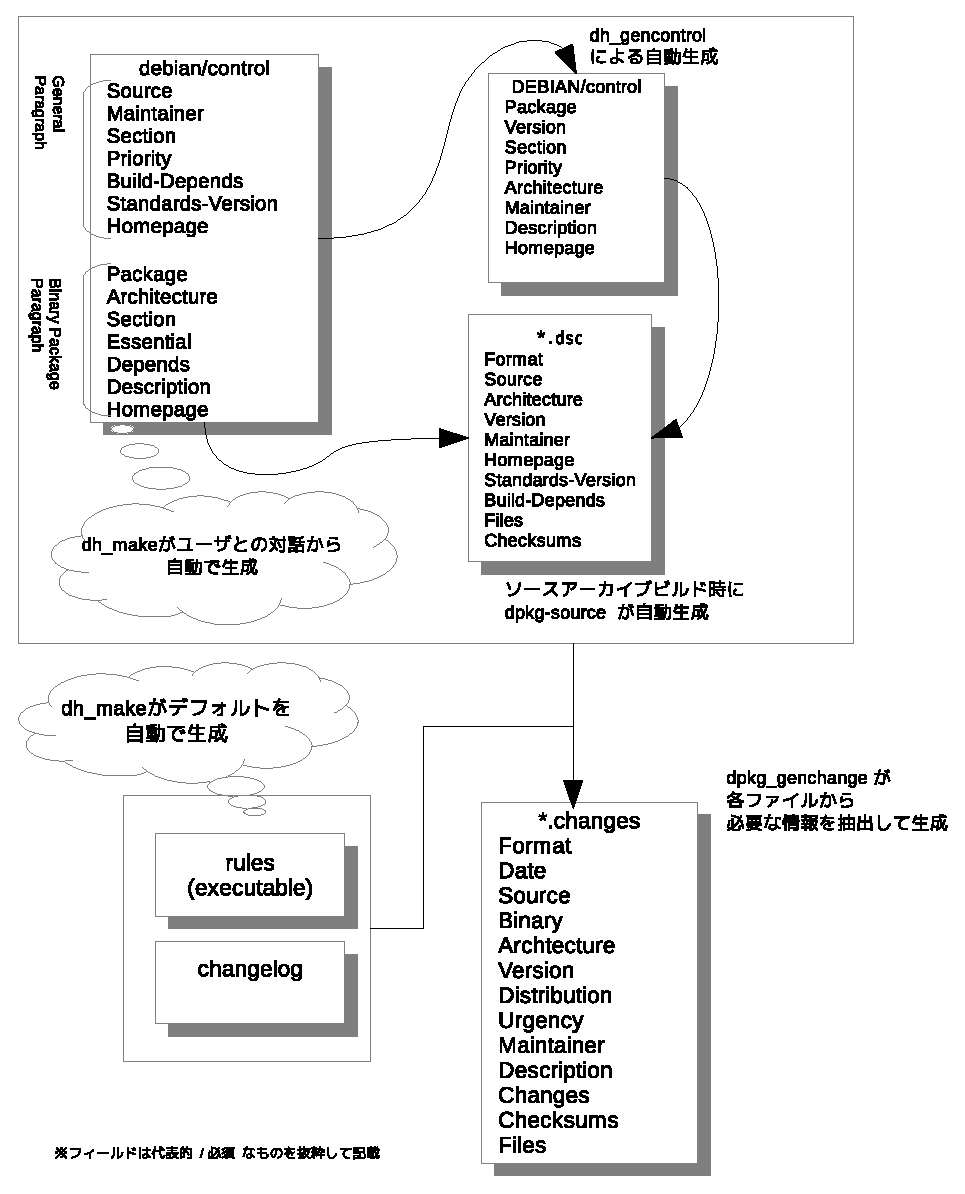
\includegraphics[scale=0.5]{image201203/control.eps}
\end{figure}

\clearpage
\dancersection{$B:#8e$NM=Dj(B}{Debian JP}

\subsection{$B<!2s(B}

$B<!2s$O!"(B2012$BG/(B4$B7n(B22$BF|$KJ!Eg6hL1%;%s%?!<$G9T$$$^$9!#(B\\
$BH/I=$K$D$$$F$OL$Dj$G$9$N$G!"$_$J$5$^$NH/I=$r$*BT$A$7$F$*$j$^$9!#(B

% $B:};R$K$9$k$?$a$K!"(B4$B$NG\?t$K$9$kI,MW$,$"$k!#(B
% $B$=$N$?$a$ND4@0(B
% \dancersection{$B%a%b(B}{}
% \mbox{}\newpage
% \mbox{}\newpage

\printindex
 \cleartooddpage

 \begin{minipage}[b]{0.2\hsize}
  \rotatebox{90}{\fontsize{80}{80} {\gt $B4X@>(B Debian $BJY6/2q(B} }
 \end{minipage}
 \begin{minipage}[b]{0.8\hsize}

 \vspace*{15cm}
 \rule{\hsize}{1mm}
 \vspace{2mm}
 \includegraphics[width=2cm]{image200502/openlogo-nd.eps}
 \noindent \Large \bf Debian $BJY6/2q;qNA(B\\ \\
 \noindent \normalfont \debmtgyear{}$BG/(B\debmtgmonth{}$B7n(B\debmtgdate{}$BF|(B \hspace{5mm}  $B=iHGBh(B1$B:~H/9T(B\\
 \noindent \normalfont $B4X@>(B Debian $BJY6/2q(B $B!JJT=8!&0u:~!&H/9T!K(B\\
 \rule{\hsize}{1mm}
 \end{minipage}

\end{document}
